\begin{figure}[t!]
    \centering
    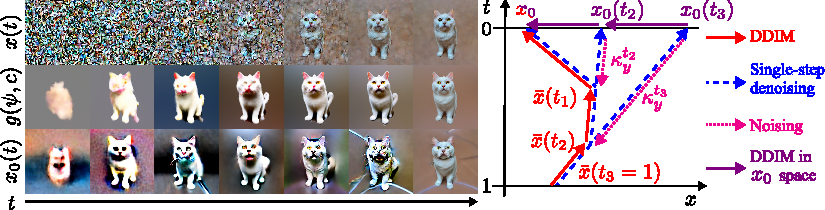
\includegraphics[width=0.99\linewidth]{figs/reparametrization_intuition.pdf}
    \vspace{-.1in}
    \caption{
        Left: Evolution of variables in Score Distillation with time. The top row depicts how noisy images $x(t)$ evolve during 2D generation; the middle row shows evolution of a NeRF for 3D generation; and the bottom row shows how the single step denoised variable $x_0(t)$ changes with $t$.
        Right: Each \textcolor{red}{step of DDIM} steps toward a  denoised image. This can be seen as a \textcolor{blue}{step to $x_0(t)$} and a \textcolor{magenta}{step back to a slightly less noisy image}. Through a change-of-variables we obtain a \textcolor{violet}{process on $x_0(t)$}.
        }
    \label{fig:evolution}
    \vspace{-.1in}
\end{figure}


\textbf{Discrepancy in image sampling.} 
Beyond the lack of formal justification of \cref{eq:dreamfusion}, in practice SDS results 
are over-saturated and miss details for high CFG values, while they are blurry for low CFG values. 
%
To illustrate this phenomenon, \cref{fig:teaser} shows a simple experiment, inspired by~\cite{wang2024prolificdreamer}: 
We replace the volumetric representation in \cref{eq:dreamfusion} with an image $g_{2D}(\psi_{2D}, c) := \psi_{2D} \in \mathbb R^{N\times N}$.
%
In this case, SDS becomes an image generation algorithm that can be compared to other sampling algorithms like DDIM~\cite{song2020denoising}. 
%
Even in this 2D setting, SDS fails to generate sharp details, while DDIM with the same underlying diffusion model produces photorealistic results, motivating our derivation below.

\textbf{Why not use DDIM as guidance?} 
Given the experiment above, a natural question to ask is if it is possible to directly
use DDIM's update direction from \cref{eq:DDIM} as SDS guidance in \cref{eq:dreamfusion} to update the 3D representation. 
%
The problem with this approach lies in the discrepancy between the training data of the denoising model and the images generated
by rendering the current 3D representation. 
More specifically, the denoising network expects an image with a certain level of noise corresponding to time $t$ as defined by the forward (noising) diffusion process,
whereas renderings of 3D representations $g(\psi, c)$ evolve from a blurry cloud to a well-defined sample (\cref{fig:evolution} left).


\textbf{Evolution of $x_0(t)$.} 
Instead of seeing DDIM as a denoising process defined on the space of noisy images $x(t)$, we reparametrize it to a new variable: 
\begin{equation}
    \label{eq:x0t}
    x_0(t) \triangleq \bar{x}(t) - \sigma(t) \epsilon_\theta^{t} \bigl( x(t), y\bigr).
\end{equation}
In words, $x_0(t)$ is the noisy image at time $t$ denoised with a single step of noise prediction.
Empirically, the evolution of $x_0(t)$ is similar to the evolution of $g(\psi, c)$---from blurry to sharp.
The left side of \cref{fig:evolution} compares these processes.
%
This similarity motivates us to rewrite \cref{eq:DDIM} in terms of $x_0(t)$, and to understand SDS as applying similar updates to the renderings of its 3D representation.

\textbf{Reparametrizing DDIM.} 
\label{section:reparametrization}
\Cref{fig:evolution} (right) shows schematically how the DDIM update to $\bar{x}(t)$ alternates between denoising to obtain $x_0(t)$ and adding the predicted noise back to get a cleaner $\bar{x}(t - \tau)$.
%
Based on the intuition above, we reorder the steps, adding noise to
$x_0(t)$ and then denoising to estimate $x_0(t - \tau)$.
%
Consider neighboring time points $t$ and $t - \tau < t$ 
in discretized DDIM \cref{eq:DDIM_disc} (lower time means less noise). We rewrite \cref{eq:DDIM_disc} using the definition of $x_0(t)$ from \cref{eq:x0t} to find
\begin{equation}
    \label{eq:exact_update}
    x_0(t - \tau) =  x_0(t) - \sigma(t - \tau) \left[ 
                 \epsilon_\theta^{t - \tau}\bigl(x(t - \tau), y\bigr)
               - \epsilon_\theta^{t       }\bigl(x(t       ), y\bigr)
            \right] \text{,}
\end{equation}
which is consistent with the intuition behind SDS: improving an image 
involves perturbing the current image and then denoising it with a better noise estimate.
We cannot directly apply \cref{eq:exact_update} to SDS in 3D, since it depends on $x(t)$; if we think of $x_0(t)$ as similar to a rendering of the 3D representation for some camera angle, it is unclear how to obtain a consistent set of preimages $x(t)$ at each step of 3D generation. From \cref{eq:x0t}, however, $x(t)$ should satisfy the following fixed point equation:
\begin{equation}
    \label{eq:fixed_eq_x}
        x(t) = \sqrt{\alpha(t)} x_0(t) + \sqrt{1 - \alpha(t)} \epsilon_\theta^{t} \bigl( x(t), y\bigr) \text{,}
\end{equation}
or rewritten in terms of noise $\epsilon = [ x(t) - \sqrt{\alpha(t)} x_0(t) ] / \sqrt{1 - \alpha(t)} $:%\justin{this step lost me}
\begin{equation}
    \label{eq:fixed_eq_eps}
        \epsilon = \epsilon_\theta^{t} \bigl( \sqrt{\alpha(t)} x_0(t) + \sqrt{1 - \alpha(t)} \epsilon, y\bigr) \text{.}
\end{equation}

Define $\kappa^t_y\bigl(x_0(t)\bigr) = \epsilon$ as a solution of 
this equation given $x_0(t)$. Then, we can write:
\begin{equation}
    \label{eq:kappa_deriv}
        \epsilon_\theta^{t} \bigl( x(t), y\bigr) = \kappa^{t}_y\bigl(x_0(t) \bigr)%\\
        \textrm{\quad and\quad}
        x(t - \tau) = \sqrt{\alpha(t - \tau)} x_0(t) + \sqrt{1 - \alpha(t - \tau)} \kappa^{t}_y\bigl(x_0(t)\bigr) \text{.}
\end{equation}

Thus, \cref{eq:exact_update} turns into:
\begin{equation}
    \label{eq:exact_update_kappa}
    x_0(t \!-\! \tau) =  x_0(t) \!-\! \sigma(t \!-\! \tau) \bigl[  
                 \underbrace{
                    \epsilon_\theta^{t - \tau} \bigl( 
                        \overbrace{
                            \sqrt{\alpha(t \!-\! \tau)} x_0(t) \!+\! \sqrt{1 \!-\! \alpha(t \!-\! \tau)} \kappa^{t}_y\bigl(x_0(t)\bigr)
                        }^{\text{$x_0$ noised with $\kappa^t_y$ to time $t - \tau$}}
                        , y
                    \bigr)
                }_{\text{predicted noise}}
               \!-\! 
               \underbrace{
                \kappa^{t}_y\bigl(x_0(t)\bigr)
               }_{\text{noise sample $\kappa^t_y$}}\!\!\!
            \bigr]\! \text{.}
\end{equation}

We can already see that the structure of \cref{eq:exact_update_kappa} is very similar to the SDS update rule in \cref{eq:dreamfusion}.
Note that the update direction in \cref{eq:exact_update_kappa} is the same as in the SDS update rule in \cref{eq:dreamfusion}, where $\kappa^t_y$ plays the role of the random noise sample $\epsilon$. 
We could use it as a guidance for the 3D generative process in SDS by replacing $\epsilon$ in \cref{eq:dreamfusion} with $\kappa^t_y(x_0(t)).$ 
In practice, however, it is hard to solve \cref{eq:fixed_eq_eps},  as $\epsilon_\theta^{t}$ is high-dimensional and nonlinear.
%
In an unconstrained 2D generation, $\kappa^t_y$ can be cached from a previous denoising step, matching the update step to DDIM exactly as in \cref{fig:teaser}c.
%
In 3D, however, this is impossible due to the simultaneous optimization of multiple views and projections to the space of viable 3D shapes.
%
Below we show that a na\"ive approximation replacing $\kappa^t_y$ with a Gaussian yields SDS, and we will propose alternatives that are more faithful to the derivation above. 


\textbf{SDS as a special case.} 
From \cref{eq:exact_update_kappa}, to get a cleaner image, we need to bring the 
current image to time $t$ with noise sample $\kappa^t_y$, 
denoise the obtained image, and then subtract the difference between added 
and predicted noise from the initial image.
%
A coarse approximation of $\kappa^t_y$ uses i.i.d.\ random noise 
$\kappa_{\textrm{SDS}}(x_0(t)) \sim \mathcal{N}(0, I)$, matching the forward process by which diffusion adds noise. This choice of $\kappa_{\textrm{SDS}}$ precisely matches the update rule \cref{eq:exact_update_kappa} to the SDS guidance in \cref{eq:dreamfusion}.

\textbf{ISM as a special case.}
The main update formula in Interval Score Matching (ISM)~\cite{liang2023luciddreamer} is a particular case of \cref{eq:exact_update_kappa}, where $\kappa^t_y$ is obtained via DDIM inversion without conditioning on the text prompt $y$.
As demonstrated in \cref{sec:sdi}, DDIM inversion approximates a solution of \cref{eq:exact_update_kappa}, explaining the improved performance of ISM.
However, our analysis suggests that an even better-performing $\kappa^t_y$ should incorporate the text prompt $y$, which further improves the results and avoids over-saturation.

 